\section{Functional Requirements}
\subsection{Introduction}

\subsubsection{Scope}
The subsystem should be implemented with in the currents AutoMart system and should not replace it. The subsystem needs to provide features that will help AutoMart reduce the number of poor and irrelevant advertisements on their website.

The subsystem needs to accept an image and return information about the image. The information should include the following, car existence in the image, colour of the car and the rating of the image. The advert image upload will depend on the image rating. If the image rating is too low, it will be prevented from being uploaded. 

The subsystem performs three tests on the advert image in order to calculate the rating. The first test checks if the image uploaded contains a car. If the system detects a car in the image, the test is seen as successful and goes on to the next test. If the system does not detect a car in the image, further image tests come to a halt. A relevant message will be stored in the image object and the system proceeds onto the next image. The second test determines the colour of the car. AutoMart currently has seventeen colour buckets that used to describe the colour of the car. The system needs to calculate which colour bucket is the closest to the cars colour. After the colour bucket has been determined, it stores the colour  into the image object. Further testing can proceed even if the system was unable to determine the colour. Third test tries to determine the make of the car. The system uses textual data to help it determine the make, as determining the make blindly will be to time consuming. The detected make is stored in the image object and proceeds onto the final test. If the system was unable to detect a make of the car, the testing comes to a halt. Final test tries to determine the model of the car. It uses previous test information to help it determine the model of the car. If the model is determined the information is stored into the image object and proceeds onto the next image.

After all the images have been put through the tests, the image objects representing the images are  put through a final set of tests to ensure that there is no information conflict. The system first checks if all the objects have the same colour. If  there is conflict it tries to resolve it by checking how many object have the same colour and how many don't. The information is also compared against the textual data. If the colour differs between the objects or it differs from the textual data the system will conclude that the images are representing different cars. This would mean that the advertisement is invalid and further testing will halt, and the advert will not be allowed to be uploaded to the system. The second test compares all the make information. If conflict is encountered the same principles as with in the colour conflict will be applied. Finally, the last test compares all the model information. The model testing will be more lenient than the first two tests. If the models differ in most of the objects and also differ from textual data, the textual data will be used to state the model of the car.

After all the test have been passed or halted unexpectedly, the system will provide relevant error messages or informative messages that were encountered during the image testing. The user will have a chance to fix any of the errors a system encountered. If the test were successful  initially or after the user has fixed the errors the advert will be allowed to be uploaded to the system.

Because the system is working with ever changing product, the system needs to accommodate for learning new cars. This way the system will never become unusable at a later stage as it will be able to stay updated with new cars.
\pagebreak
\begin{figure}[h!]
  \caption{High Level System Use Case Diagram.}
  \centering
	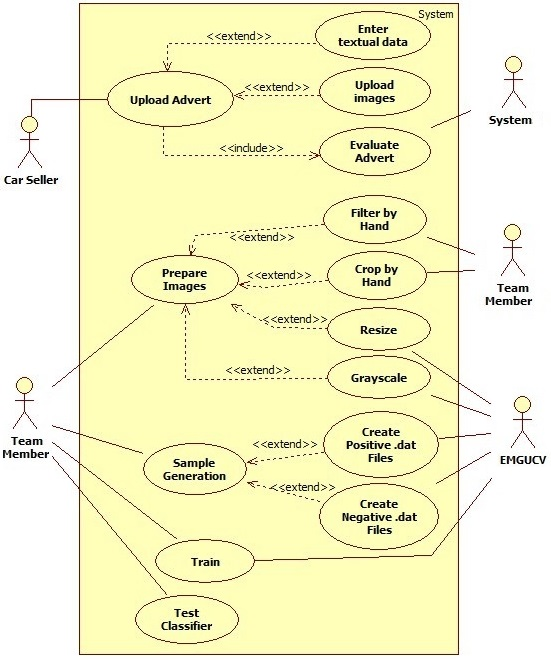
\includegraphics{HighLevelSystemUseCase.jpg}
\end{figure}

\subsubsection{Limitations}
The system may be limited on model recognition, as sometimes it is not possible to distinguish the model of the car by only face value properties that are given by an image. Therefore the system may not be able to determine the model of the car correctly every time.

\subsubsection{Exclusions}
The system should only be implemented to work with cars and should not consider for the existence of any other motor vehicles such as motorcycles and trucks.

\subsection{Required Functionality}
\begin{figure}[h!]
  \caption{Detect Car Low Level Use Case Diagram.}
  \centering
	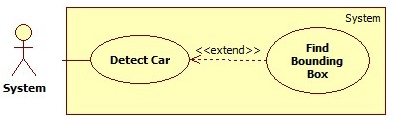
\includegraphics{DetectCarLowLevelUseCaseDiagram.jpg}
\end{figure}

\begin{figure}[h!]
  \caption{Describe Car Low Level Use Case Diagram.}
  \centering
	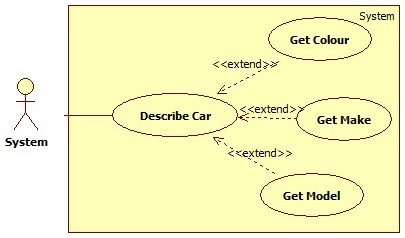
\includegraphics{DescribeCarLowLevelUseCaseDiagram.jpg}
\end{figure}

\begin{figure}[h!]
  \caption{Generate Rating Low Level Use Case Diagram.}
  \centering
	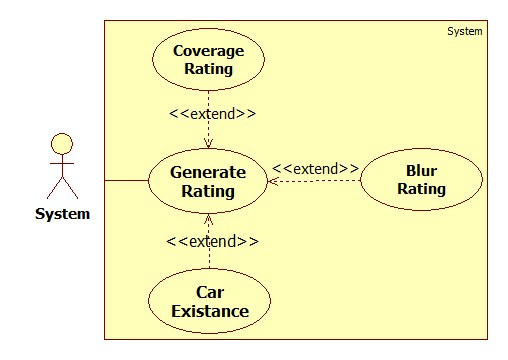
\includegraphics{GenerateRatingLowLevelUseCaseDiagram.jpg}
\end{figure}

\subsection{Use Cases}
\textbf{Detect Car Subsystem}\\
\begin{tabular}{ | l | l |}
	\hline
  	\multicolumn{2}{| c |}{\textbf{Find Bounding Box}} \\
  	\hline
  	\multicolumn{2}{| c |}{Determines if the car exists in the photo and returns co-ordinates of the box containing the car.}\\
	\hline
	Priority & Critical \\	
  	\hline
  	Pre-Conditions & A valid image needs to be provided.\\
  	\hline
 	Post-Conditions & Car detection status provided.\\
  	\hline
\end{tabular}\\
\\
\\
\textbf{Describe Car Subsystem}\\
\begin{tabular}{ | l | l | }
	\hline
  	\multicolumn{2}{| c |}{\textbf{Determine Colour}} \\
  	\hline
  	\multicolumn{2}{| c |}{Determines the colour of the car and finds the closest colour bucket.}\\
	\hline
	Priority & Important \\	
  	\hline
  	Pre-Conditions & A car needs to exist in the bounding box.\\
  	\hline
 	Post-Conditions & Colour of the car is determined.\\
  	\hline
\end{tabular}\\
\\
\\
\begin{tabular}{ | l | l | }
	\hline
  	\multicolumn{2}{| c |}{\textbf{Determine Make}} \\
  	\hline
  	\multicolumn{2}{| c |}{Determines the make of the car.}\\
	\hline
	Priority & Nice to have \\	
  	\hline
  	Pre-Conditions & A car needs to exist in the bounding box. A make classifier needs to exist.\\
  	\hline
 	Post-Conditions & Make status determined.\\
  	\hline
\end{tabular}\\
\\
\\
\begin{tabular}{ | l | l | }
	\hline
  	\multicolumn{2}{| c |}{\textbf{Determine Model}} \\
  	\hline
  	\multicolumn{2}{| c |}{Determines the model of the car.}\\
	\hline
	Priority & Nice to have \\	
  	\hline
  	Pre-Conditions & A car needs to exist in the bounding box.\\
  	\hline
 	Post-Conditions & Model status determined.\\
  	\hline
\end{tabular}\\
\\
\\
\textbf{Generate Rating Subsystem}\\
\begin{tabular}{ | l | l | }
	\hline
  	\multicolumn{2}{| c |}{\textbf{Get Colour Value}} \\
  	\hline
  	\multicolumn{2}{| c |}{Returns a weighted value based whether the colour has been determined or not.}\\
	\hline
	Priority & Important \\	
  	\hline
  	Pre-Conditions & Use case "Determine Colour" was executed successfully.\\
  	\hline
 	Post-Conditions & Colour value successfully calculated and returned.\\
  	\hline
\end{tabular}\\
\\
\\
\begin{tabular}{ | l | l | }
	\hline
  	\multicolumn{2}{| c |}{\textbf{Get Make Value}} \\
  	\hline
  	\multicolumn{2}{| c |}{Returns a weighted value based whether the make has been determined or not.}\\
	\hline
	Priority & Important \\	
  	\hline
  	Pre-Conditions & Use case "Determine Make" was executed successfully.\\
  	\hline
 	Post-Conditions & Make value successfully calculated and returned.\\
  	\hline
\end{tabular}\\
\\
\\
\begin{tabular}{ | l | l | }
	\hline
  	\multicolumn{2}{| c |}{\textbf{Get Model Value}} \\
  	\hline
  	\multicolumn{2}{| c |}{Returns a weighted value based whether the model has been determined or not.}\\
	\hline
	Priority & Important \\	
  	\hline
  	Pre-Conditions & Use case "Determine Model" was executed successfully.\\
  	\hline
 	Post-Conditions & Model value successfully calculated and returned.\\
  	\hline
\end{tabular}\\
\\
\\
\begin{tabular}{ | l | l | }
	\hline
  	\multicolumn{2}{| c |}{\textbf{Calculate Blur}} \\
  	\hline
  	\multicolumn{2}{| c |}{Stretches the bounding box to 480x320 pixels and calculates and returns the blur value.}\\
	\hline
	Priority & Important \\	
  	\hline
  	Pre-Conditions & Bounding box exists.\\
  	\hline
 	Post-Conditions & Blur value successfully calculated and returned.\\
  	\hline
\end{tabular}\\
\\
\\
\begin{tabular}{ | l | l | }
	\hline
  	\multicolumn{2}{| c |}{\textbf{Calculate Position}} \\
  	\hline
  	\multicolumn{2}{| c |}{Determines where in the photo the car placed, and returns the value based on the position.}\\
	\hline
	Priority & Important \\	
  	\hline
  	Pre-Conditions & Bounding box exists.\\
  	\hline
 	Post-Conditions & Car position value successfully calculated and returned.\\
  	\hline
\end{tabular}\\
\\
\\
\begin{tabular}{ | l | l | }
	\hline
  	\multicolumn{2}{| c |}{\textbf{Calculate Coverage}} \\
  	\hline
  	\multicolumn{2}{| c |}{Calculates the coverage the car occupies in the photo.}\\
	\hline
	Priority & Important \\	
  	\hline
  	Pre-Conditions & Bounding box exists.\\
  	\hline
 	Post-Conditions & Car coverage  value successfully calculated and returned.\\
  	\hline
\end{tabular}\\
\\
\\
\begin{tabular}{ | l | l | }
	\hline
  	\multicolumn{2}{| c |}{\textbf{Calculate Resolution}} \\
  	\hline
  	\multicolumn{2}{| c |}{.}\\
	\hline
	Priority & Important \\	
  	\hline
  	Pre-Conditions & Valid image provided.\\
  	\hline
 	Post-Conditions & Photo resolution value successfully calculated and returned.\\
  	\hline
\end{tabular}\\
\\
\\
\begin{tabular}{ | l | l | }
	\hline
  	\multicolumn{2}{| c |}{\textbf{Calculate Contrast}} \\
  	\hline
  	\multicolumn{2}{| c |}{Calculates contrast ratio of the photo.}\\
	\hline
	Priority & Important \\	
  	\hline
  	Pre-Conditions & Valid image provided.\\
  	\hline
 	Post-Conditions & Photo contrast value successfully calculated and returned.\\
  	\hline
\end{tabular}\\
\pagebreak
\subsection{Process Specifications}
\begin{figure}[h!]
  \caption{Activity diagram of FindBoundingBox}
  \centering
	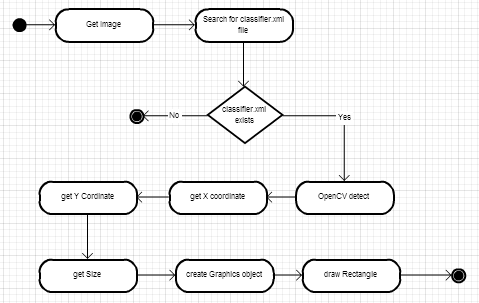
\includegraphics{activity.PNG}
\end{figure}
